% =============================================================================
% COPYRIGHT AND DISCLAIMER
% =============================================================================
% This file is provided as a convenience template for competition participants.
% By using it, you accept full responsibility for compliance with all applicable
% copyright, licensing, and usage rules of the Association for Computing
% Machinery (ACM) and of any LaTeX packages you load (including, without
% limitation, the "acmart" document class and related ACM materials).
%
% Consult ACM's official publication, template, and copyright policies before
% using this setup for any purpose other than this competition. Do not assume
% that this template may be reused, redistributed, or submitted elsewhere
% without independently verifying ACM's current rules.
%
% Use of the "acmart" class, the "sigconf" option, or ACM-style formatting in
% this template does NOT mean that this report, this competition, its organizers,
% or any resulting PDF is sponsored, endorsed, affiliated with, or published by
% ACM. ACM trademarks and branding remain the property of ACM.
%
% Template packages live in preamble.tex.
% Citations live in main.bib. Edit this file with your paper content.
% =============================================================================

\documentclass[sigconf]{acmart}
% =============================================================================
% Template setup — participants normally do not edit this file.
% Author content belongs in main.tex; citations belong in main.bib.
% \documentclass lives in main.tex so Overleaf does not treat this file as root.
% =============================================================================

% --- Competition / non-ACM-submission friendly rights metadata -------------
\setcopyright{none}
\settopmatter{printacmref=false}
\acmConference[Kaggle Competition]{Filament Segmentation Challenge}{2026}{\href{https://www.kaggle.com/competitions/filament-segmentation-2026}{kaggle.com/competitions/filament-segmentation-2026}}
\acmBooktitle{Competition Report}
\acmDOI{}
\acmISBN{}

% --- Author guidance text --------------------------------------------------
% \guide{...} is gray italic while \guideStyletrue; omitted from the PDF if false.
% Flip the switch in main.tex after % =============================================================================
% Template setup — participants normally do not edit this file.
% Author content belongs in main.tex; citations belong in main.bib.
% \documentclass lives in main.tex so Overleaf does not treat this file as root.
% =============================================================================

% --- Competition / non-ACM-submission friendly rights metadata -------------
\setcopyright{none}
\settopmatter{printacmref=false}
\acmConference[Kaggle Competition]{Filament Segmentation Challenge}{2026}{\href{https://www.kaggle.com/competitions/filament-segmentation-2026}{kaggle.com/competitions/filament-segmentation-2026}}
\acmBooktitle{Competition Report}
\acmDOI{}
\acmISBN{}

% --- Author guidance text --------------------------------------------------
% \guide{...} is gray italic while \guideStyletrue; omitted from the PDF if false.
% Flip the switch in main.tex after % =============================================================================
% Template setup — participants normally do not edit this file.
% Author content belongs in main.tex; citations belong in main.bib.
% \documentclass lives in main.tex so Overleaf does not treat this file as root.
% =============================================================================

% --- Competition / non-ACM-submission friendly rights metadata -------------
\setcopyright{none}
\settopmatter{printacmref=false}
\acmConference[Kaggle Competition]{Filament Segmentation Challenge}{2026}{\href{https://www.kaggle.com/competitions/filament-segmentation-2026}{kaggle.com/competitions/filament-segmentation-2026}}
\acmBooktitle{Competition Report}
\acmDOI{}
\acmISBN{}

% --- Author guidance text --------------------------------------------------
% \guide{...} is gray italic while \guideStyletrue; omitted from the PDF if false.
% Flip the switch in main.tex after \input{preamble}.
%
% Do not use \guide{...} for \email{...}.
\usepackage{xcolor}
\newif\ifguideStyle
\guideStyletrue
\newcommand{\guide}[1]{%
  \ifguideStyle
    {\color{gray!65}\itshape #1}%
  \fi
}

% --- Math ------------------------------------------------------------------
% Do NOT load amssymb (or amsfonts): acmart already loads newtxmath, which
% defines the same symbols (e.g. \Bbbk) and causes a conflict on Overleaf.
% amsmath is already provided by acmart; mathtools extends it.
\usepackage{mathtools}

% --- Figures ---------------------------------------------------------------
% graphicx is already loaded by acmart
\usepackage{subcaption}

% --- Tables ----------------------------------------------------------------
% booktabs is already loaded by acmart
\usepackage{tabularx}
\usepackage{multirow}

% --- Bibliography style is set in main.tex (ACM-Reference-Format) ----------
.
%
% Do not use \guide{...} for \email{...}.
\usepackage{xcolor}
\newif\ifguideStyle
\guideStyletrue
\newcommand{\guide}[1]{%
  \ifguideStyle
    {\color{gray!65}\itshape #1}%
  \fi
}

% --- Math ------------------------------------------------------------------
% Do NOT load amssymb (or amsfonts): acmart already loads newtxmath, which
% defines the same symbols (e.g. \Bbbk) and causes a conflict on Overleaf.
% amsmath is already provided by acmart; mathtools extends it.
\usepackage{mathtools}

% --- Figures ---------------------------------------------------------------
% graphicx is already loaded by acmart
\usepackage{subcaption}

% --- Tables ----------------------------------------------------------------
% booktabs is already loaded by acmart
\usepackage{tabularx}
\usepackage{multirow}

% --- Bibliography style is set in main.tex (ACM-Reference-Format) ----------
.
%
% Do not use \guide{...} for \email{...}.
\usepackage{xcolor}
\newif\ifguideStyle
\guideStyletrue
\newcommand{\guide}[1]{%
  \ifguideStyle
    {\color{gray!65}\itshape #1}%
  \fi
}

% --- Math ------------------------------------------------------------------
% Do NOT load amssymb (or amsfonts): acmart already loads newtxmath, which
% defines the same symbols (e.g. \Bbbk) and causes a conflict on Overleaf.
% amsmath is already provided by acmart; mathtools extends it.
\usepackage{mathtools}

% --- Figures ---------------------------------------------------------------
% graphicx is already loaded by acmart
\usepackage{subcaption}

% --- Tables ----------------------------------------------------------------
% booktabs is already loaded by acmart
\usepackage{tabularx}
\usepackage{multirow}

% --- Bibliography style is set in main.tex (ACM-Reference-Format) ----------


% Guide styling: \guideStyletrue = show gray italic hints; \guideStylefalse = omit them
% \guideStyletrue
\guideStylefalse

\begin{document}

\title[Agreement-Weighted Detection and Crop Refinement]{Agreement-Weighted Detection and Crop Refinement for Solar Filament Instance Segmentation}  % Replace this with your title
\subtitle{A Solution to the Solar Filament Segmentation Challenge 2026} % DO NOT CHANGE


\author{Ishan Sharma}
\affiliation{%
  \institution{Dalhousie University}  % <- Optional (remove if you are not currently affiliated with any institute)
  \city{Halifax}
  \country{Canada}
}
\email{ishansharma1320@gmail.com}   % <- Replace with your own email

\begin{abstract}
    This report describes our solution to the Solar Filament Segmentation Challenge~2026, a Kaggle competition on automatic segmentation of solar filaments in GONG H-$\alpha$ observations. We use a two-stage cascade: an ensemble of 20 YOLO11 box detectors proposes one box per filament, and five crop U-Nets draw one mask per box at native resolution, so instances can never merge or overlap. The detector is trained to predict how many annotators drew each filament, and its confidence is scaled by that agreement class, which aligns the ranking with the pooled Panoptic Quality (PQ) metric. Under 5-fold cross-validation grouped by image and scored against every annotator record, the final ensemble reaches PQ $0.451$ (single model $0.450$, 95\% CI $[0.441, 0.460]$), against $0.340$ for one human annotator scored against another; public leaderboard PQ is $0.40$. We also report what did not help (higher resolution, larger or transformer detectors, temporal sequences, self-training, copy-paste), and why: the remaining errors sit on faint filaments whose annotation is itself inconsistent.
\end{abstract}

\maketitle

% ==================================== %
%              INTRODUCTION            %
% ==================================== %
\section{Introduction}
    This report goes over the details of our submitted solution to the Solar Filament Segmentation Challenge~2026 \cite{filament-segmentation-2026}. The challenge, launched on July~10,~2026, is organized by the Earth-Space AI Research (ESAIR) Lab\footnote{\href{https://www.esairlab.com/home}{www.esairlab.com/}}. This challenge utilizes the MAGFiLO dataset for evaluation of the segmentation algorithms \cite{ahmadzadeh2024dataset}. Since the metric is Panoptic Quality \cite{kirillov2019panoptic} with a strict IoU~$>0.5$ match, pooled over every annotator's record, a filament split into two pieces scores zero and costs one false negative plus two halves of a false positive. Our design therefore puts instance integrity first and treats the keep/drop decision for each filament as the main problem. Our contributions are: (i) a detect-then-refine cascade that guarantees one non-overlapping mask per detection; (ii) agreement-class labels, which teach the detector which filaments most annotators draw; and (iii) a measured account of the remaining error, including a comparison with human inter-annotator agreement. Code, weights and a reproduction notebook are public \cite{repo2026}.

% ==================================== %
%              METHODOLOGY             %
% ==================================== %
\section{Methodology}\label{sec:methodology}

\begin{figure*}[t]
  \centering
  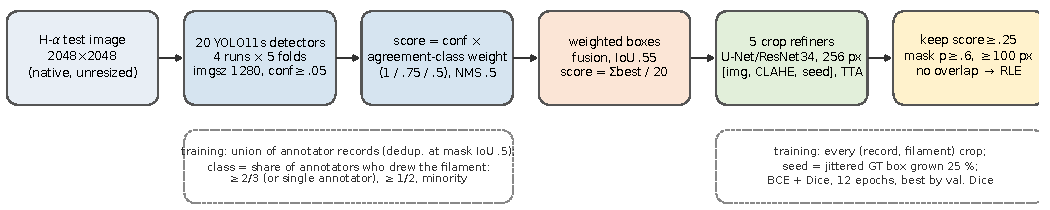
\includegraphics[width=\textwidth]{fig_pipeline.pdf}
  \caption{End-to-end inference pipeline (top) and how its two trained stages are supervised (dashed). All geometry is kept in native $2048{\times}2048$ pixel coordinates; masks are never resampled.}
  \label{fig:pipeline}
\end{figure*}

\paragraph{Data and splits.} The 707 training images carry 1{,}154 annotator records (411 images with one annotator, 145 with two, 151 with three) and 8{,}199 filament polygons. We use 5-fold cross-validation \emph{grouped by physical image}, so the records of one observation never straddle training and validation (fixed seed, 141--142 images per fold). All model selection uses out-of-fold (OOF) predictions scored exactly like the organisers' self-evaluation notebook: PQ pooled over all 1{,}154 records. No external labels or pretrained filament models are used; the detectors and refiners start from public ImageNet/COCO weights.

\paragraph{Stage 1: agreement-weighted detector.} We train YOLO11s \cite{yolo11_ultralytics} on the native JPEGs at input size 1280 for 40 epochs per fold (vertical and horizontal flips, default mosaic/HSV augmentation). Labels are the \emph{union} of all records of an image: filaments from different annotators are clustered at mask IoU~$\geq 0.5$ (at most one filament per record per cluster) and each cluster is represented by its most central member. Each box gets a class from its annotator support $s$ (the share of the image's annotators who drew it): \emph{high} ($s\geq 2/3$, and every box of a single-annotator image), \emph{half} ($s\geq 1/2$) or \emph{minority}. This yields 4{,}552 / 869 / 1{,}027 boxes. Including minority filaments as their own class, instead of dropping them, forces the classification loss to separate agreement levels. At inference we use class-agnostic NMS (IoU~0.5) and score each box as $\mathrm{conf}\times w_c$ with $w=(1, 0.75, 0.5)$. The motivation is decision-theoretic: under pooled PQ a predicted filament with expected match IoU $u$, drawn by a fraction $q$ of the annotators, raises PQ only if $q\,u > \mathrm{PQ}/2$ (the PQ analogue of \cite{lipton2014thresholding}), so the ranking should follow expected agreement.

\paragraph{Stage 2: crop refiner.} For each box, a U-Net \cite{ronneberger2015unet} with a ResNet34 encoder \cite{he2016resnet} (\texttt{segmentation\_models\_pytorch} \cite{iakubovskii2019smp}) segments a square crop of side $\max(256, 1.4\times$ the box's long side$)$, centred on the box; crops larger than 256~px are resized to 256 and the probability map is resized back. The input has three channels: the image, its CLAHE-equalised copy, and a \emph{seed} (the box grown by 25\% per side, filled) that tells the network which filament to draw when several share the crop. The refiner is trained on every (record, filament) pair of the training folds, about 6.5k crops per fold, with jittered ground-truth boxes as seeds (shift up to 15\%, scale 0.8--1.25), BCE+Dice loss, 12 epochs (OneCycle, lr $3{\cdot}10^{-4}$), keeping the epoch with the best validation Dice.

\paragraph{Ensembling and post-processing.} The final entry fuses 20 detectors: the 5 fold models of four training runs that differ only in detector recipe (v9: single-class, v10: YOLO11m, v11: extra archive views, v13: agreement classes). Per image, their boxes are merged by weighted boxes fusion \cite{solovyev2021wbf} at IoU~0.55; a fused box's score is the sum of each detector's best matching score divided by 20, so boxes found by few detectors are demoted. The five v13 refiners average their 4-flip test-time-augmented probabilities in every fused box. Instances are then built in score order: keep boxes with score~$\geq 0.25$, threshold the probability at 0.6, keep only the components touching the seed, drop masks under 100~px, drop a mask if more than half of it is already claimed by a higher-scored instance, and clip the rest, so no two instances share a pixel. All three thresholds were selected on OOF PQ. Figure~\ref{fig:examples} shows typical results on held-out images.

\paragraph{Reproducibility.} The 25 weight files (937~MB) are committed to the repository with SHA-256 checksums; a notebook loads them and regenerates the submitted CSV on CPU in about 1.7~h. All 1{,}218 instances it produces are bit-identical to the submitted file.

\begin{figure*}[t]
  \centering
  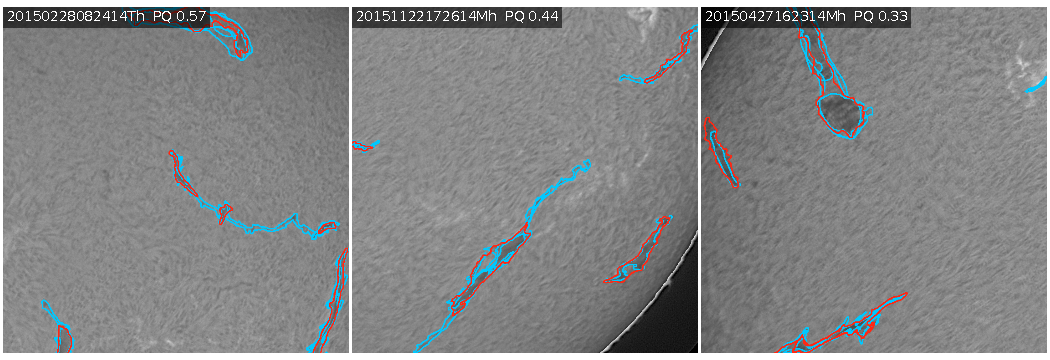
\includegraphics[width=\textwidth]{fig_examples.pdf}
  \caption{Out-of-fold predictions (red) against all three annotators' outlines (cyan) on three held-out images at the 85th, 50th and 15th percentile of per-image PQ. Each panel is a $760{\times}760$ native-pixel window. Typical failures (right): faint or fragmented filaments drawn by only some annotators.}
  \label{fig:examples}
\end{figure*}

% ==================================== %
%              EVALUATION              %
% ==================================== %
\section{Evaluation}\label{sec:evaluation}

\paragraph{Strategy.} We report pooled OOF PQ over all 1{,}154 annotator records of the 707 training images, its decomposition $\mathrm{PQ}=\mathrm{SQ}\times\mathrm{RQ}$ (segmentation and recognition quality), per-fold variation, and a 95\% bootstrap interval (1{,}000 resamples of images). As a human reference we score each annotator's masks against every other annotator of the same image (296 images with 2--3 annotators). Public-leaderboard PQ consistently ran $\approx 0.05$ below OOF across all our submissions, and moved by exactly the OOF-predicted amount in controlled probes (e.g.\ dilating every mask by 1~px: OOF $-0.02$, LB $-0.01$), so we used OOF for every decision and the leaderboard only for confirmation.

\begin{table}[t]
  \caption{Main results (OOF over all annotator records unless noted).}
  \label{tab:main}
  \footnotesize
  \setlength{\tabcolsep}{3.2pt}
  \begin{tabular}{lccc}
    \toprule
    & PQ & SQ & RQ \\
    \midrule
    Single model (v13), pooled & 0.450 & 0.689 & 0.653 \\
    \quad 95\% bootstrap CI & [.441, .460] & [.686, .692] & [.640, .667] \\
    \quad per-fold mean $\pm$ s.d. & 0.450 $\pm$ 0.014 & -- & -- \\
    Final ensemble (20 detectors) & \textbf{0.451} & 0.687 & 0.657 \\
    Final ensemble, public LB & 0.40 & -- & -- \\
    \midrule
    Annotator vs.\ annotator & 0.340 & 0.634 & 0.536 \\
    \bottomrule
  \end{tabular}
\end{table}

\begin{figure*}[t]
  \centering
  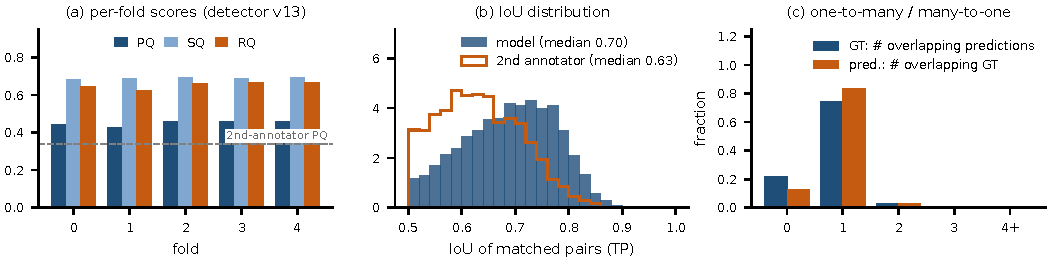
\includegraphics[width=\textwidth]{fig_eval.pdf}
  \caption{(a) Per-fold PQ, SQ and RQ of the single v13 model; dashed: one annotator scored against another. (b) IoU of matched (TP) pairs: model vs.\ a second annotator. (c) For each ground-truth filament, the number of predictions overlapping it (blue), and for each prediction, the number of ground-truth filaments it overlaps (orange); ``1'' is the clean one-to-one case.}
  \label{fig:eval}
\end{figure*}

\paragraph{Results.} Table~\ref{tab:main} and Figure~\ref{fig:eval} summarise performance. The model's masks agree with an annotator better than a second annotator does: median matched IoU is 0.70 vs.\ 0.63 (median Dice 0.82), and SQ is 0.689 vs.\ 0.634. Relations are overwhelmingly one-to-one: 84\% of predictions and 75\% of ground-truth filaments overlap exactly one partner; one-to-many and many-to-one cases are about 3\% each, so fragmentation and merging are rare. Errors are dominated by existence decisions: 22\% of ground-truth filaments are not touched by any prediction, and 13\% of predictions touch no annotation. Relative to a second annotator, and per true positive, our single detector (v9) makes half as many outline disagreements (0.23 vs.\ 0.45) and half as many unannotated detections (0.17 vs.\ 0.33), but 16\% more complete misses (0.38 vs.\ 0.33).

\begin{table}[t]
  \caption{What moved OOF PQ (one change at a time; full log in the repository).}
  \label{tab:ablation}
  \small
  \begin{tabular}{lc}
    \toprule
    Change & OOF PQ \\
    \midrule
    Semantic U-Net + connected components (1024~px) & 0.410 \\
    \quad + native 2048~px input & 0.391 \\
    Detect-then-refine cascade (YOLO11s, 1024~px) & 0.444 \\
    \quad + union labels, 1280~px native input & 0.445 \\
    \quad + agreement classes (v13) & \textbf{0.450} \\
    \quad + fusion of 20 detectors (final) & \textbf{0.451} \\
    \midrule
    \multicolumn{2}{l}{\emph{No gain over the row above (within $\pm$0.004 unless noted):}} \\
    \quad YOLO11m; refiner hard negatives / objectness head & 0.441--0.445 \\
    \quad RF-DETR detector (one fold, vs.\ 0.436) & 0.420 \\
    \quad archive frames as extra labelled views & 0.434 \\
    \quad self-training on archive frames; EffNet-B3 refiner & 0.448 \\
    \quad copy-paste augmentation & 0.448 \\
    \bottomrule
  \end{tabular}
\end{table}

\paragraph{Ablations and negative results.} Table~\ref{tab:ablation} lists every change we tested. Two changes mattered. The cascade (+0.034) replaced pixel-level merging with per-object existence decisions, cutting false positives by 42\%. Agreement classes (+0.004 alone, +0.006 with fusion) improved the ranking: at an equal number of true positives the detector produces about 300 fewer unannotated detections. Changes that improve what the detector \emph{sees} did not help. These were resolution, capacity, transformer detectors (RF-DETR was also 6$\times$ slower on a T4), extra images and augmentation. We also used public GONG frames as training-time sequences (the hosts allow this for training only). Detector candidates that no annotator drew persist across other telescopes and over 6~h of solar rotation as often as drawn ones. Temporal persistence predicts annotation worse than detector confidence does (AUC 0.62 vs.\ 0.73). The unannotated candidates are real solar features that annotators chose to skip, in line with MAGFiLO's own guidance to omit small, faint or grouped filaments, which annotators applied inconsistently.

\paragraph{Strengths, weaknesses, improvements.} \emph{Strengths:} instances are guaranteed non-overlapping and rarely fragmented; masks exceed inter-annotator agreement; inference needs only the test image and is exactly reproducible on CPU. \emph{Weaknesses:} recall on faint, short filaments drawn by a minority of annotators (35--58\% box recall vs.\ 76--91\% on consensus filaments) is the main remaining error. Since persistence, capacity and resolution do not separate these cases, we see the remaining gap as mostly annotation variability rather than model error. A self-matching oracle of our design bounds achievable PQ near 0.55 on multi-annotator images, against our 0.44 there. \emph{Improvements:} per-annotator modelling (e.g.\ learned annotator reliabilities) to predict agreement directly; calibrating the keep threshold per image from expected agreement; and training on more images annotated by several experts, which would sharpen the agreement targets the detector learns from.

% ==================================== %
%            ACKNOWLEDGMENT            %
% ==================================== %
\section{Acknowledgment}\label{sec:acknowledgment}
    % Do not change
    The organization of the Filament Segmentation Challenge 2026 is partially supported by the U.S. National Science Foundation (NSF) under Grant No. 2209912 and 2433781, directorate for Computer and Information Science and Engineering (CSE), and Office of Advanced Cyberinfrastructure (OAC), and Grant No. 2511630, AST Division Of Astronomical Sciences and MPS Directorate for Mathematical and Physical Sciences.

    The Filament Segmentation Challenge 2026 is sponsored by the U.S. National Science Foundation (NSF) National Solar Observatory (NSO).

    This work utilizes GONG data obtained by the NSO Integrated Synoptic Program, managed by the National Solar Observatory, which is operated by the Association of Universities for Research in Astronomy (AURA), Inc. under a cooperative agreement with the National Science Foundation and with contribution from the National Oceanic and Atmospheric Administration. The GONG network of instruments is hosted by the Big Bear Solar Observatory, High Altitude Observatory, Learmonth Solar Observatory, Udaipur Solar Observatory, Instituto de Astrofísica de Canarias, and Cerro Tololo Interamerican Observatory.

\bibliographystyle{ACM-Reference-Format}
\bibliography{main}

\end{document}
